\documentclass[12pt]{book}

\usepackage{mathptm,times,color}
\usepackage[pdftex]{graphicx}
\usepackage{multirow}
\usepackage{bezier}
\usepackage{rotating}
\usepackage{longtable}
\usepackage{amsmath}
\usepackage{xfrac}
\usepackage{array}
\usepackage{units}
\usepackage{fix-cm}
\usepackage{xspace}
\usepackage{makeidx} % Create index at end of document
\usepackage[nottoc,notlof,notlot]{tocbibind} % Put the bibliography and index in the ToC
\usepackage{datetime}
\newdateformat{mydate}{\monthname[\THEMONTH] \THEYEAR}

\usepackage{listings}
\usepackage{textcomp}
\definecolor{lbcolor}{rgb}{0.96,0.96,0.96}
\lstset{
    %backgroundcolor=\color{lbcolor},
    tabsize=4,
    rulecolor=,
    language=Fortran,
        basicstyle=\footnotesize\ttfamily,
        upquote=true,
        aboveskip={\baselineskip},
        belowskip={\baselineskip},
        columns=fixed,
        extendedchars=true,
        breaklines=true,
        breakatwhitespace=true,
        frame=none,
        showtabs=false,
        showspaces=false,
        showstringspaces=false,
        identifierstyle=\ttfamily,
        keywordstyle=\color[rgb]{0,0,0},
        commentstyle=\color[rgb]{0,0,0},
        stringstyle=\color[rgb]{0,0,0},
}

\usepackage{wrapfig}
\usepackage{morefloats}

\newcolumntype{L}[1]{>{\raggedright\let\newline\\\arraybackslash\hspace{0pt}}m{#1}}
\newcolumntype{C}[1]{>{\centering\let\newline\\\arraybackslash\hspace{0pt}}m{#1}}
\newcolumntype{R}[1]{>{\raggedleft\let\newline\\\arraybackslash\hspace{0pt}}m{#1}}

\IfFileExists{../Bibliography/gitrevision.tex}
{\input{../Bibliography/gitrevision}}
{\newcommand{\gitrevision}{unknown} }

\usepackage{framed}
\newcommand{\graybox}[1]{
\begin{shaded}#1\end{shaded}
}

\usepackage{changepage}

\renewcommand{\bibname}{References}

% dummy change to force revision update

%\usepackage{eso-pic}
%\usepackage{graphicx}
%\usepackage{color}
%\usepackage{type1cm}


%\makeatletter
%   \AddToShipoutPicture{%
%     \setlength{\@tempdimb}{.5\paperwidth}%
%    \setlength{\@tempdimc}{.5\paperheight}%
%   \setlength{\unitlength}{1pt}%
%  \put(\strip@pt\@tempdimb,\strip@pt\@tempdimc){%
%     \makebox(0,0){\rotatebox{45}{\textcolor[gray]{0.75}{\fontsize{8cm}{8cm}\selectfont{DRAFT}}}}}}
%\makeatother

\definecolor{linknavy}{rgb}{0,0,0.50196}
\definecolor{linkred}{rgb}{1,0,0}
\definecolor{linkblue}{rgb}{0,0,1}
\definecolor{shadecolor}{rgb}{0.9,0.9,0.9}

\usepackage[pdftex,
        colorlinks=true,
        urlcolor=linkblue,     % \href{...}{...} external (URL)
        citecolor=linkred,     % citation number colors
        linkcolor=linknavy,    % \ref{...} and \pageref{...}
        pdfproducer={pdflatex},
        pagebackref,
        pdfpagemode=UseNone,
        bookmarksopen=true,
        plainpages=false,
        verbose]{hyperref}

\usepackage{siunitx}
\sisetup{
    detect-all = true,
    input-decimal-markers = {.},
    input-ignore = {,},
    inter-unit-product = \ensuremath{{}\cdot{}},
    multi-part-units = repeat,
    number-unit-product = \text{~},
    per-mode = fraction,
    separate-uncertainty = true,
}

% CFAST Version String
\newcommand{\cfastversion}{7.2.3}

% commands to use for "official" cover and title pages
% see smokeview verification guide to see how they are used

\newcommand{\logosigs}{
\begin{minipage}[b]{6.5in}
\flushright{
\includegraphics[height=1.05in]{FIGURES/nistident}}
\end{minipage}
}

\newcommand{\titlesigs}
{
\small
\begin{flushright}
U.S. Department of Commerce \\
{\em Penny Pritzker, Secretary} \\
\hspace{1in} \\
National Institute of Standards and Technology \\
{\em Willie May, Acting Under Secretary of Commerce for Standards and Technology and Acting Director}
\end{flushright}
}

\newcommand{\headerA}[1]{
\begin{flushright}
\fontsize{20}{24}\selectfont
\bf{NIST Technical Note #1}
\end{flushright}
}


\newcommand{\headerB}[1]{
\begin{flushright}
\fontsize{28}{33.6}\selectfont
\bf{#1}
\end{flushright}
}

\newcommand{\headerC}[1]{
\vspace{.15in}
\begin{flushright}
\fontsize{12}{14}\selectfont
#1
\end{flushright}
}

\newcommand{\headerD}[1]{
\begin{flushright}
\fontsize{12}{14}\selectfont
This publication is available free of charge from: \\
http://dx.doi.org/10.6028/NIST.TN.#1
\end{flushright}
}

\newcommand{\coden}[1]{
\vspace*{\fill}
\begin{flushright}
\fontsize{12}{14}\selectfont
\textbf{National Institute of Standards and Technology Technical Note #1 \\
Natl. Inst. Stand. Technol. Tech. Note #1, \pageref{last_page} pages (\mydate\today) \\
CODEN: NTNOEF \\
\vspace{\baselineskip}
This publication is available free of charge from: \\
http://dx.doi.org/10.6028/NIST.TN.#1}
\end{flushright}
}



\setlength{\textwidth}{6.5in}
\setlength{\textheight}{9.0in}
\setlength{\topmargin}{0.in}
\setlength{\headheight}{0.in}
\setlength{\headsep}{0.in}
\setlength{\parindent}{0.25in}
\setlength{\oddsidemargin}{0.0in}
\setlength{\evensidemargin}{0.0in}

\newcommand{\vecy}{\mathbf{y}}
\newcommand{\vecF}{\mathbf{F}}
\newcommand{\rd}{\mathrm{d}}
\newcommand{\brackets}[1]{ { \left( {#1} \right) } }
\newcommand{\dcydt}[1]{\rd{#1}/\rd t}
\newcommand{\dbydt}[1]{\frac{\rd {#1}}{\rd t}}
\newcommand{\dbydx}[1]{\frac{\partial {#1}}{\partial x}}
\newcommand{\ddt}{\frac{\rd}{\rd t}}
\newcommand{\superscript}[1]{\ensuremath{^{\textnormal{\scriptsize \hbox{#1}}}}}
\newcommand{\subscript}[1]{\ensuremath{_{\textnormal{\scriptsize \hbox{#1}}}}}

\newcommand{\textct}[1]{\texttt{\small #1}}

\newcommand{\cp}{{\rm c}_{\rm p}}
\newcommand{\cv}{{\rm c}_{\rm v}}

\newcommand{\trho}{\tilde{\rho}}
\newcommand{\chia}{\chi_{\rm a}}
\newcommand{\chir}{\chi_{\rm r}}
\newcommand{\dph}{{\delta\phi}}
\newcommand{\dth}{{\delta\theta}}
\newcommand{\tp}{\tilde{p}}
\newcommand{\dQ}{\dot{Q}}
\newcommand{\dQc}{\dot{Q}_{\rm c}}
\newcommand{\dQr}{\dot{Q}_{\rm r}}
\newcommand{\Dh}{\Delta H}
\newcommand{\DhO}{\Delta H_\OTWO}
\newcommand{\Tp}{T_{\rm p}}
\newcommand{\Tu}{T_{\rm u}}
\newcommand{\Tl}{T_{\rm l}}
\newcommand{\Ti}{T_i}
\newcommand{\Tw}{\mathbf{T}_{\rm w}}
\newcommand{\Ts}{T_{\rm s}}
\newcommand{\Tg}{T_{\rm g}}
\newcommand{\TL}{T_{\rm L}}
\newcommand{\Vu}{V_{\rm u}}
\newcommand{\Vl}{V_{\rm l}}
\newcommand{\Vi}{V_i}
\newcommand{\doh}{\dot{h}}
\newcommand{\dhl}{\dot{h}_{\rm l}}
\newcommand{\dhu}{\dot{h}_{\rm u}}
\newcommand{\dmal}{\dot{m}_{\rm l}}
\newcommand{\dmau}{\dot{m}_{\rm u}}
\newcommand{\dq}{\dot{q}}
\newcommand{\dqc}{\dot{q}_{\rm c}}
\newcommand{\dqr}{\dot{q}_{\rm r}}
\newcommand{\dql}{\dot{q}_{\rm l}}
\newcommand{\dqu}{\dot{q}_{\rm u}}
\newcommand{\dqi}{\dot{q}_i}
\newcommand{\dm}{\dot{m}}
\newcommand{\dme}{\dot{m}_{\rm e}}
\newcommand{\dmp}{\dot{m}_{\rm p}}
\newcommand{\dml}{\dot{m}_{\rm l}}
\newcommand{\dmu}{\dot{m}_{\rm u}}
\newcommand{\dmi}{\dot{m}_i}
\newcommand{\dmf}{\dot{m}_{\rm f}}
\newcommand{\ml}{m_{\rm l}}
\newcommand{\mmu}{m_{\rm u}}
\newcommand{\mi}{m_i}

\newcommand{\be}{\begin{equation}}
\newcommand{\ee}{\end{equation}}

\newcommand{\RE}{\hbox{Re}}
\newcommand{\LE}{\hbox{Le}}
\newcommand{\PR}{\hbox{Pr}}
\newcommand{\PE}{\hbox{Pe}}
\newcommand{\NU}{\hbox{Nu}}
\newcommand{\SC}{\hbox{Sc}}
\newcommand{\SH}{\hbox{Sh}}
\newcommand{\WE}{\hbox{We}}

\newcommand{\COTWO}{{\tiny \hbox{CO}_2}}
\newcommand{\OTWO}{{\tiny \hbox{O}_2}}
\newcommand{\CO}{{\tiny \hbox{CO}}}
\newcommand{\HTWOO}{{\tiny \hbox{H}_2\hbox{O}}}
\newcommand{\NTWO}{{\tiny \hbox{N}_2}}
\newcommand{\F}{{\tiny \hbox{F}}}
\newcommand{\So}{{\tiny \hbox{S}}}
\newcommand{\M}{{\tiny \hbox{M}}}
\newcommand{\HCN}{{\tiny \hbox{HCN}}}
\newcommand{\HCl}{{\tiny \hbox{HCl}}}
\newcommand{\Hy}{{\tiny \hbox{H}}}
\newcommand{\C}{{\tiny \hbox{C}}}
\newcommand{\N}{{\tiny \hbox{N}}}
\newcommand{\Oh}{{\tiny \hbox{O}}}
\newcommand{\Cl}{{\tiny \hbox{Cl}}}

\newcommand{\asqh}{$A_T/A\sqrt{h}$}
\newcommand{\degc}{$^{\circ}$C\xspace}
\newcommand{\degf}{$^{\circ}$F\xspace}

\newcommand{\dx}{\delta x}
\newcommand{\dy}{\delta y}
\newcommand{\dz}{\delta z}
\newcommand{\dt}{\delta t}

\newcommand{\ha}{\frac{1}{2}}
\newcommand{\ft}{\frac{4}{3}}
\newcommand{\ot}{\frac{1}{3}}
\newcommand{\fofi}{\frac{4}{5}}
\newcommand{\of}{\frac{1}{4}}
\newcommand{\twth}{\frac{2}{3}}

\newcommand{\ct}{\tt\small}

\newcommand{\rb}[1]{\raisebox{1.5ex}[0pt]{#1}}

\newcommand{\erf}{\hbox{erf}}



\begin{document}

\bibliographystyle{unsrt}

\frontmatter

\pagestyle{empty}


\begin{minipage}[t][9in][s]{6.5in}

\headerA{1889v4\\}

\headerB{
CFAST -- Consolidated Fire \\
 and Smoke Transport \\
 (Version 7) \\
 Volume 4: Software Quality Assurance \\
}

\headerC{
   Richard D. Peacock \\
}

\vfill

\headerD{1889v4}

\vfill

\logosigs

\end{minipage}

\newpage

\hspace{5in}

\newpage

\begin{minipage}[t][9in][s]{6.5in}

\headerA{1889v4\\}

\headerB{
CFAST -- Consolidated Fire \\
 And Smoke Transport \\
 (Version 7) \\
 Volume 4: Software Quality Assurance \\
}

\headerC{
   Richard D. Peacock \\
}

\headerD{1889v4}

\headerC{
\flushright{\mydate\today\\
CFAST Version \cfastversion \\
\emph{GIT Revision:}~\gitrevision}}

\vfill

\flushright{
\includegraphics[width=1.2in]{FIGURES/doc} }

\titlesigs

\end{minipage}


\newpage

\frontmatter

\pagestyle{plain}
\setcounter{page}{3}

\chapter{CFAST Developers}

The Consolidated Model of Fire and Smoke Transport (CFAST) and Smokeview are the products of a collaborative effort led by the National Institute of Standards and Technology (NIST). Its developers and contributors are listed below.

\vspace{0.3in}

\begin{flushleft}

Principal Developers of CFAST  \\ [0.2in]

Richard Peacock, NIST \\
Glenn Forney, NIST \\
Paul Reneke, NIST \\
Kevin McGrattan, NIST \\
Walter Jones \\ [0.3in]

Principal Developer of Smokeview  \\ [0.2in]

Glenn Forney, NIST \\ [0.3in]

Contributors \\ [0.2in]

Kristopher Overholt, Continuum Analytics, Austin, Texas, USA \\ [0.3in]
Jason Floyd, Jensen Hughes, Baltimore, Maryland, USA \\

\end{flushleft}


\chapter{About the Developers}

\begin{description}

\item[Richard Peacock] is a chemical engineering in the Fire Research Division of NIST. He received a bachelor of science degree from the Clark School of Engineering of the University of Maryland in 1973. He joined the NIST staff in 1974 (then the National Bureau of Standards) and has worked on real-scale testing and the development and validation of fire models, most notably CFAST.

\item[Glenn Forney] is a computer scientist in the Fire Research Division of NIST.  He received a bachelor of science degree in mathematics from Salisbury State College and a master of science and a doctorate in mathematics from Clemson University.  He joined NIST in 1986 (then the National Bureau of Standards) and has since worked on developing tools that provide a better understanding of fire phenomena, most notably Smokeview, an advanced scientific software tool for visualizing Fire Dynamics Simulation data.

\item[Paul Reneke] is a computer scientist in the Fire Research Division of NIST.  He received a bachelor of science degree in mathematical sciences from Clemson Univerity and a master of science degree in applied mathematics from The Johns Hopkins University. He joined NIST in 1990. He has worked on the development of user interfaces, graphics and improved numerics in fire models, notably CFAST. His research interests include sensitivity analysis and validation of fire models.

\item[Kevin McGrattan] is a mathematician in the Fire Research Division of NIST. He received a bachelor of science degree from the School of Engineering and Applied Science of Columbia University in 1987 and a doctorate at the Courant Institute of New York University in 1991. He joined the NIST staff in 1992 and has since worked on the development and validation of fire models, most notably the Fire Dynamics Simulator.

\item[Walter Jones] was a physicist at NIST (now retired). He received a bachelor of arts degree in physics from Oberlin College and a doctorate in physics from the University of Maryland. He was the original developer of the CFAST model. In addition to the development of fire models, he has worked on smart fire alarms and smoke control for naval vessels.

\end{description}





\chapter{Preface}

The purpose of this document is to describe the policies and procedures for developing and maintaining CFAST. Such a document is commonly referred to as a {\em Software Quality Assurance Plan}.  This includes

\begin{itemize}
    \item Relevant documentation for the model: Description of the theoretical basis of the model \cite{CFAST_Tech_Guide_7}\, instructions for its are contained in a separate user's guide \cite{CFAST_Users_Guide_7}, and model assessment information is contained in a separate verification and validation guide \cite{CFAST_Valid_Guide_7}.

    \item Description of the development process for the model.

    \item Control and tracking of the source code using a centralized project repository on GitHub.

    \item An automated build, verification, validation, and regression testing process then helps the CFAST development team by performing automatic error checking and collecting performance and accuracy statistics between CFAST revisions.

    \item Details of the review process used by the developers and NIST to ensure the quality of the model and related publications.

\end{itemize}

\chapter{Disclaimer}

The US Department of Commerce makes no warranty, expressed or implied, to users of CFAST, and accepts no responsibility for its use. Users of CFAST assume sole responsibility under Federal law for determining the appropriateness of its use in any particular application; for any conclusions drawn from the results of its use; and for any actions taken or not taken as a result of analysis performed using these tools.

Users are warned that CFAST is intended for use only by those competent in the fields of fluid dynamics, thermodynamics, heat transfer, combustion, and fire science, and is intended only to supplement the informed judgment of the qualified user. The software package is a computer model that may or may not have predictive capability when applied to a specific set of factual circumstances. Lack of accurate predictions by the model could lead to erroneous conclusions with regard to fire safety. All results should be evaluated by an informed user.

Throughout this document, the mention of computer hardware or commercial software does not constitute endorsement by NIST, nor does it indicate that the products are necessarily those best suited for the intended purpose.

\coden{1889v4}


\chapter{Acknowledgments}

\label{acksection}

CFAST was originally developed by Walter Jones, formerly of NIST.

Continuing support for CFAST is via internal funding at NIST. In addition, support is provided by other agencies of the U.S. Federal Government, most notably the Nuclear Regulatory Commission (NRC) and the Department of Energy (DOE). The NRC Office of Nuclear Regulatory Research has funded key validation experiments, the preparation of the CFAST manuals, and the continuing development of sub-models that are of importance in the area of nuclear power plant safety. Special thanks to Mark Salley and David Stroup for their support. Support to refine the software development and quality assurance process for CFAST has been provided by the U.S. Department of Energy. The assistance of Subir Sen and Debra Sparkman is gratefully acknowledged.

The idea for this document originated with Jason Floyd, a co-developer of FDS and practicing engineer at Jensen Hughes. He readily saw the need for a clear description of the process of developing and maintaining FDS and Smokeview. This plan adapts the FDS process for the CFAST model.  Bryan Klein, currently with Thunderhead Engineering, Inc., and Kristopher Overholt, currently with Continuum Analytics instituted a number of the internet tools that are described in the Guide, including the source code repository, issue tracking system, and discussion group sites.


\tableofcontents

\listoffigures


\mainmatter

\chapter{Overview}

This document describes the processes used during the development and deployment of the Consolidated Fire and Smoke Transport model (CFAST).  This software quality assurance (SQA) plan is intended to guide the planning for modifications to the model, provide required reviews for both software and associated documentation of the model, define testing to be conducted prior to the release of an updated model, describe problem reporting and resolution procedures, and ensure all records, source code, and released software is kept available for the life of the code.  While this report and many of our practices follow the ASTM International Standard 1355-05, ``Standard Guide for Evaluating the Predictive Capability of Deterministic Fire Models'' \cite{ASTM:E1355} which has been used extensively to guide the documentation, verification, and validation of the model, other standards have been followed as well.  Most notably, Institute of Electrical and Electronics Engineers (IEEE) standard for software quality assurance, IEEE 730-2002 \cite{IEEE:730} best practices in important areas of software quality assurance and guides the structure and content of this plan.

The volumes that make up the CFAST documentation are based in part on ASTM E 1355, {\em Standard Guide for Evaluating the Predictive Capability of Deterministic Fire Models}~\cite{ASTM:E1355}. ASTM~E~1355 outlines the process of assessing the accuracy of a fire model. Volumes~1 through 3 are the result of this evaluation process. The main purpose of the present volume is to describe the process by which the model software is developed and maintained. A model such as CFAST cannot remain static. As progress is made in fire science, the model needs to be updated and improved, but still shown to reliably predict the kinds of phenomena for which it was originally designed.

CFAST is intended for use only by those competent in the field of fire safety and is intended only to supplement the informed judgment of the qualified user. The software package is a computer model which has limitations based on the way it is used, and the data used for calculations. All results should be evaluated by a qualified user.

The SQA process and requirements outlined in this document apply specifically to the CFAST and is focused on ensuring the quality of the numerical predictions of the model.  The user interface that may be used to develop input for the model is included in this process to insure that changes to the model are reflected in the user interface and in the data files created by the user interface for use by the model.  Of course, users must ensure that the input files developed for the simulations accurately reflect the desired model inputs, whether developed using the supplied user interface, another third-party interface, or manually input with a spreadsheet or text editor program.  Documentation of these inputs is included as part of the model documentation outlined below.

Documentation and configuration management for its companion visualization program Smokeview, is included in the documentation for the Fire Dynamics Simulator (FDS) and Smokeview \cite{FDS_Configuration_Guide_6}.

\IfFileExists{../Bibliography/model_description.tex}{

\section{Model Type}

CFAST is a two-zone fire model that predicts the thermal environment caused by a fire within a compartmented structure. Each compartment is divided into an upper and lower gas layer (zone in the term zone fire model refers to the layers being modeled). The fire drives combustion products from the lower to the upper layer via the plume. The temperature within each layer is uniform, and its evolution in time is described by a set of ordinary differential equations derived from the fundamental laws of mass and energy conservation. The transport of smoke and heat from zone to zone is dictated by empirical correlations. Because the governing equations are relatively simple, CFAST simulations typically require a few tens of seconds of CPU time on typical personal computers.


\section{Model Version}

The first public release of CFAST was version 1.0 in June, 1990. This version was restructured from FAST~\cite{Models:FAST} to incorporate the ``lessons learned'' from the zone model CCFM developed by Cooper and Forney~\cite{Models:CCFM}. Version~2 was released as a component of Hazard~1.2 in 1994~\cite{Models:HAZARDI, Models:HAZARDI_12}. The first of the 3.x series was released in 1995 and included a vertical flame spread algorithm, ceiling jets and non-uniform heat loss to the ceiling, spot targets, and heating and burning of multiple objects (ignition by heat flux, temperature or time) in addition to multiple prescribed fires. As it evolved over the next five years, version~3 included smoke and heat detectors, suppression through heat release reduction, better characterization of flow through doors and windows, vertical heat conduction through ceiling/floor boundaries, and non-rectangular compartments. In 2000, version~4 was released and included horizontal heat conduction through walls, and horizontal smoke flow in corridors. Version~5 improved the combustion chemistry. Version 6, released in July, 2005, incorporates a more consistent implementation of vents, fire objects, and event processing and includes a graphical user interface which substantially improves its usability. Beginning with version 6, a formal revision management system was implemented to track changes to the CFAST source code. The open-source program development tools are provided by GitHub: \href{https://github.com}{\textct{https://github.com}}.

The current version of CFAST, version 7, was released in 2015.

A Wiki file, located on the CFAST web site, maintained by the developers, details the changes made for each release: \href{https://github.com/firemodels/cfast/wiki/Release-Notes}{\textct{https://github.com/firemodels/cfast/wiki/Release-Notes}}.


\section{Model Developers}

CFAST was developed and is maintained by the Fire Research Division of the National Institute of Standards and Technology. The developers are Richard Peacock, Glenn Forney, and Paul Reneke. Kevin McGrattan has participated in the changes leading to CFAST, version 7.

\section{Relevant Publications}

The manuals for CFAST consist of this Technical Reference Guide, a User's Guide~\cite{CFAST_Users_Guide_7}, a Verification and Validation Guide~\cite{CFAST_Valid_Guide_7}, and a Configuration Management Guide~\cite{CFAST_Config_Guide_7}.  The Technical Reference Guide describes the underlying physical principles. The User's Guide describes how to use the model. The Verification and Validation Guide documents sensitivity analyses, model verification, model validation, and model limitations consistent with ASTM~E1355~\cite{CFAST:ASTM:E1355}. The Configuration Management Guide documents the processes used during the development and validation of the model.

The U.S. Nuclear Regulatory Commission has published a verification and validation study of five selected fire models commonly used in support of risk-informed and performance-based fire protection at nuclear power plants~\cite{NRCNUREG1824}. In addition to an extensive study of the CFAST model, the report compares the output of several other models ranging from simple hand calculations to more complex computational fluid dynamics codes such as the Fire Dynamics Simulator (FDS) developed by the National Institute of Standards and Technology (NIST) \cite{FDS_Tech_Guide_6}.


\section{Governing Equations and Assumptions}

The governing equations of CFAST are for conservation of mass and energy within the lower and upper layers of connected compartments within a building. The momentum within any one zone is assumed to be zero.  Momentum between zones in adjacent compartments is accounted for in terms of horizontal or vent flow equations (Bernoulli's law). Other features of CFAST include:
\begin{itemize}
\item Compartment geometry: CFAST is generally limited to fire scenarios where the compartment volumes are strongly stratified. The empirical correlations contained in CFAST were developed for relatively uncluttered, flat ceilings in compartments that can be characterized as ``rooms'' as opposed to corridors or vertical shafts. There are no hard limits on what kind of compartment can or cannot be modeled in CFAST. The CFAST Validation Guide indicates the accuracy of its predictions for compartments of various aspect ratios.
\item Heat Release Rate: CFAST does not predict fire growth on burning objects. The heat release rate is specified by the user for one or more fires. There is a simple sub-model to limit the heat release based on available oxygen.
\item Radiation from fires is modeled with a simple point source approximation.  This limits the accuracy of the model within a few diameters of the fire. Calculation of radiative exchange between compartments is not modeled.
\item Mechanical ventilation is modeled by specifying volumetric flow rates into or out of compartments. The overall HVAC (heating, ventilation, air conditioning) system is not modeled.
\item Natural Ventilation and Leakage: The flow through vertical openings, like doors and windows, is modeled using the Bernoulli equation for the pressure difference between two compartments. Horizontal openings, like hatches, are treated with a single empirical correlation based on pressure and density differences between upper and lower compartments. Leakage is modeled by explicitly creating a small vertical or horizontal opening.
\item Suppression: CFAST predicts sprinkler activation based on an empirical ceiling jet correlation and activation model. A simple suppression model decreases the specified heat release rate.
\end{itemize}
The technical approach and assumptions of the model have been presented in the peer-reviewed scientific literature~\cite{Jones:1993a, Jones:1985, Jones:1984} and conference proceedings~\cite{Jones:1991}. CFAST has been reviewed and included in industry-standard handbooks such as the SFPE Handbook~\cite{Walton:2003} and referenced in specific standards, including NFPA~805~\cite{NFPA805:2004} and NFPA~551~\cite{NFPA551:2004}.

Also, all documents released by NIST are required to go through an internal editorial review and approval process. This process is designed to ensure compliance with the technical requirements, policy, and editorial quality required by NIST. The technical review includes a critical evaluation of the technical content and methodology, statistical treatment of data, uncertainty analysis, use of appropriate reference data and units, and bibliographic references. CFAST manuals are always first reviewed by a member of the Fire Research Division, then by the immediate supervisor of the author of the document, then by the chief of the Fire Research Division, and finally by a reader from outside the division. These reviewers are technical experts in the field. Once the document has been reviewed, it is then brought before the Editorial Review Board (ERB), a body of representatives from all the NIST laboratories. At least one reader is designated by the Board for each document that it accepts for review. This last reader is selected based on technical competence and impartiality. The reader is usually from outside the division producing the document and is responsible for checking that the document conforms with NIST policy on units, uncertainty and scope. This reader does not need to be a technical expert in fire or combustion.

Besides formal internal and peer review, CFAST is subjected to continuous scrutiny because it is available to the general public and is used internationally by those involved in fire safety design and postfire reconstruction. The source code for CFAST is also released publicly, and has been used at various universities worldwide, both in the classroom as a teaching tool as well as for research. As a result, flaws in the theoretical development and the computer program itself have been identified and fixed. The user base continues to serve as a means to evaluate the model, which is as important to its development as the formal internal and external peer review processes.

For each major release of CFAST, NIST has maintained a history of the source code which goes back to March 1989.  While it is not practical to reconstruct the programs for each release for use with modern software tools and computer operating systems, the source code history allows the developers to examine what changes were made at each release point. This provides detailed documentation of the history of model development and is often useful to understand the impact of changes to sub-models as the model continues to evolve.




\section{Input Data Required to Run the Model}

All of the data required to run the CFAST model reside in a single input file that the user generates. The file consists of the following information:
\begin{itemize}
\item material properties (e.g., thermal conductivity, specific heat, density, thickness, heat of combustion)
\item compartment dimensions (height, width, length)
\item construction materials of the compartment (e.g., concrete, gypsum)
\item dimensions and positions of horizontal and vertical flow openings such as doors, windows, and vents
\item mechanical ventilation specifications
\item fire properties (e.g., heat release rate, lower oxygen limit, and species production rates as a function of time)
\item sprinkler and detector specifications
\item positions, sizes, and characteristics of targets
\item specifications for visual output from the model
\end{itemize}
The input files are provided for the validation exercises described in the Validation Guide~\cite{CFAST_Valid_Guide_7}. A complete description of the input parameters can be found in the CFAST User's Guide~\cite{CFAST_Users_Guide_7}.

A comprehensive assessment of the numerical parameters (such as default time step or solution convergence criteria) and physical parameters (such as empirical constants for convective heat transfer or plume entrainment) used in CFAST is not available in one document. Instead, specific parameters have been tested in various verification and validation studies performed at NIST and elsewhere. Numerical parameters are described in this Technical Reference Guide and are subject to the internal review process at NIST, but many physical parameters are extracted from the literature and do not undergo a formal review. The model user is expected to assess the appropriateness of default values provided by CFAST and make changes to the default values, if needed.



\section{Model Results}

The output of CFAST are the sensible variables that are needed for assessing the environment in a building subjected to a fire. Once the simulation is complete, CFAST produces an output file containing all of the solution variables.  Typical outputs include (but are not limited to) the following:
\begin{itemize}
\item environmental conditions in the room (such as hot gas layer temperature; plume centerline temperature; oxygen and smoke concentration; and ceiling, wall, and floor temperatures)
\item heat transfer-related outputs to walls and targets (such as incident convective, radiative, and total heat fluxes)
\item fire intensity and flame height
\item flow velocities through vents and openings
\item detector and sprinkler activation times
\end{itemize}


\section{Model Scenarios}

While the governing transport equations are based on the fundamental conservation laws of mass and energy, the fire-specific algorithms within CFAST are based on empirical correlations. These correlations include fire plume and ceiling jet temperatures and velocities, vent flow rates, sprinkler activation, and so on. These sub-models were developed independently of each other under ideal conditions. CFAST combines these sub-models in such a way that there are no hard limits on when a particular sub-model is appropriate or not. The decision as to whether CFAST is appropriate for a given fire scenario is based primarily on the hundreds of experiments and thousands of point-to-point comparisons between CFAST and measured quantities that are included in the CFAST Validation Guide~\cite{CFAST_Valid_Guide_7}. This document includes a list of the experiments and their important physical attributes such as the nature of the fire, the aspect ratio of the compartment, the ventilation rate, and the relative location of targets. For each quantity of interest, such as upper layer temperature or target heat flux, there is a calculated bias factor and standard deviation that indicates the accuracy of the model for the particular quantity of interest which is based on measurement uncertainty. Thus, the CFAST Validation Guide indicates what fire scenarios are appropriate for CFAST, and the degree of accuracy that can be expected for a particular type of prediction.

In addition to what is included in the CFAST Validation Guide, validation studies have been performed by NIST grantees, students at universities, and engineering firms using the model.  Because each organization has its  own reasons for  validating the model, the  referenced papers and reports do not follow any particular guidelines. Some of the works only provide  a qualitative assessment  of the model,  concluding that the  model  agreement with  a  particular  experiment  is ``good''  or ``reasonable.'' Sometimes, the conclusion is that the model works well in certain cases, not as well in others. These studies are included in the survey because the references  are useful to other model users who may have a similar application  and are interested in qualitative assessment. It is important to note  that some of the papers point out flaws in early releases of CFAST that have been corrected or improved in more recent  releases. Some of  the issues raised, however,  are still subjects of  active research. Continued updates for CFAST  are greatly influenced by the feedback provided by users, often through publication of validation efforts. }{\typeout{Error: Missing file ../Bibliography/model_description.tex}}

\chapter{Configuration Management}

\section{Project Management}

CFAST is developed and maintained by the Engineering Laboratory (EL), NIST). Like all projects at NIST, a designated project leader is responsible for directing and prioritizing model development, error correction, and preparation of documentation for the model development.  The organization chart in Figure \ref{figOrgChart} provides a graphical representation of the software quality organization structure for CFAST

\begin{figure}
\begin{center}
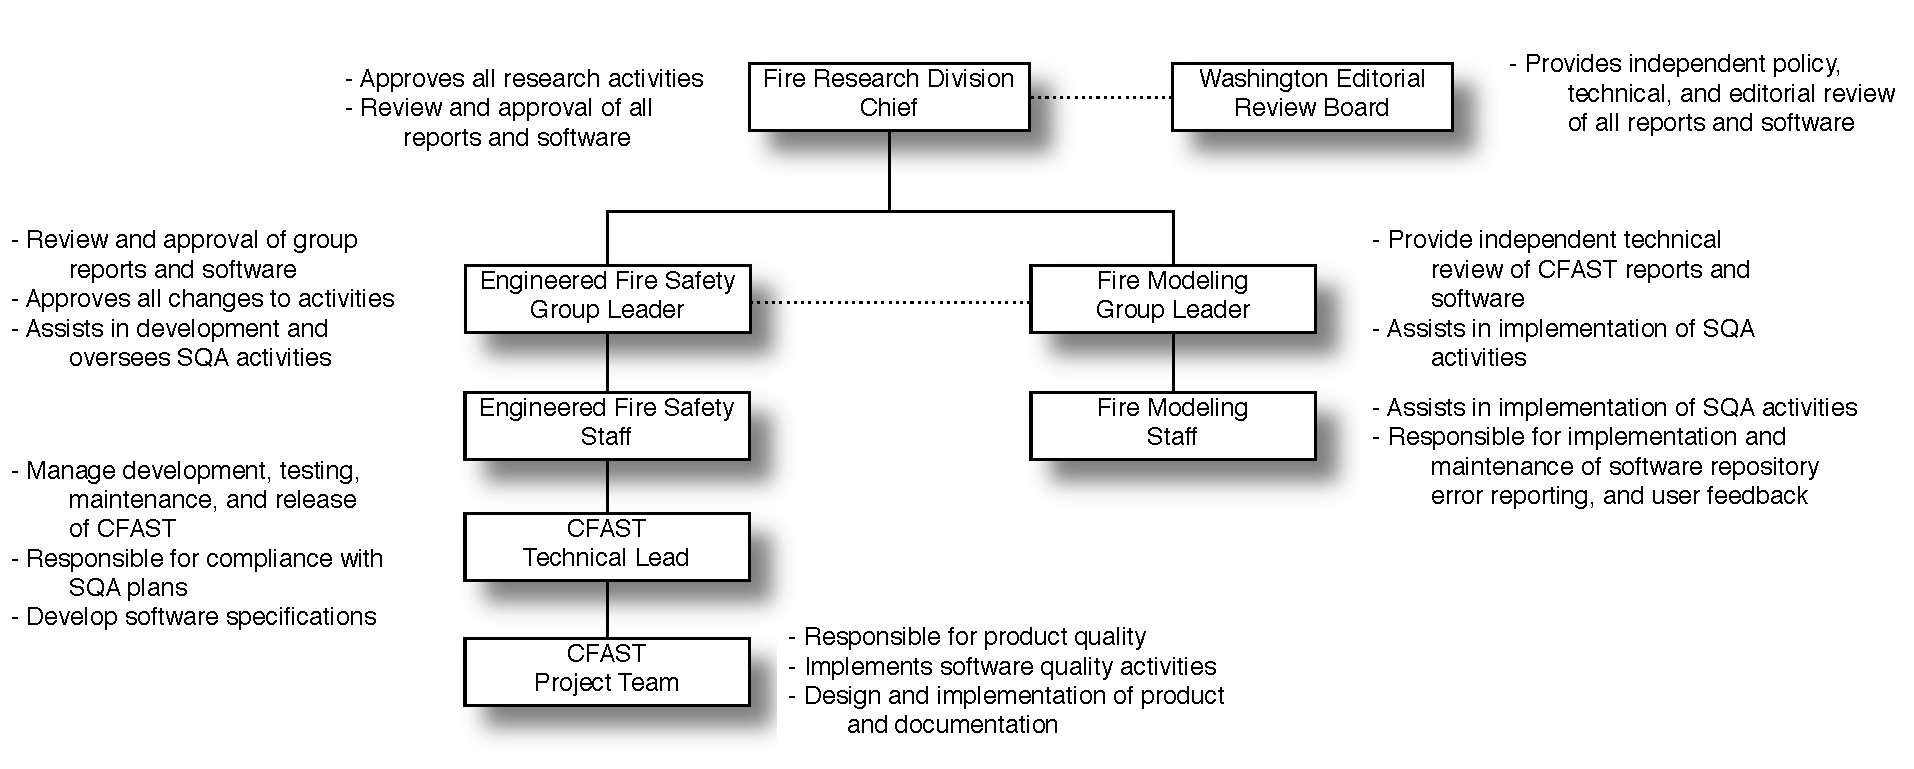
\includegraphics[width=6.5in]{FIGURES/OrgChart.pdf}\\
\end{center}
\caption{CFAST SQA Organization Structure.}
 \label{figOrgChart}
\end{figure}

Members of the CFAST team share in the development responsibilities, which include:
\begin{itemize}
\item Developing new algorithms and improving program functionality
\item Answering user questions
\item Responding to bug reports
\item Issuing periodic updates to the officially released versions of the programs
\item Maintaining the Technical Reference and Users Guides
\item Maintaining a suite of sample cases to demonstrate model use
\item Maintaining a suite of verification and validation cases to test model accuracy and reliability
\end{itemize}

Review and approval of software and documentation is part of the standard review process for any report or other product developed by NIST. A minimum of five reviews are required prior to release of reports or software, including two independent technical peer reviews, technical and management reviews at the technical workgroup and division level, and a policy review at the NIST-wide level.  This review is documented and recorded on the NIST standard form NIST 114 along with official approval notification provided to the primary author of the product.

CFAST is distributed exclusively through a NIST website dedicated to the CFAST model (http://cfast.nist.gov).  Content of the website is the responsibility of the CFAST project leader and the NIST webmaster. Additions and changes to the website are made only with the approval of the CFAST project leader after any required NIST reviews.

\section{Document Identification and Control}

Document identification and control consists of placing all project files in a central location and maintaining a record of changes to those files. The central location is known as the {\em Repository}.

CFAST and Smokeview make use of GitHub, a free service to support software development for open source applications. GitHub uses Git version control software. Under this system a centralized repository containing all project files resides on an external server.   A record of version number when a specific file was last changed is maintained. As an open source program, any individual can obtain a copy of the repository or retrieve specific versions of the repository. Only development team members can commit changes to the repository. All others must submit a “pull request” which is then reviewed by the development team for inclusion into the repository.

The current location of the CFAST repository is \href{https://github.com/firemodels/cfast}{\textct{https://github.com/firemodels/cfast}}. The repository contains more than 3000 configuration items:
\begin{enumerate}
\item CFAST source code files
\item CFAST documentation
\item Input files for software testing, verification testing, and validation testing
\item Experimental data files used for validation testing
\item Scripts and post-processing utilities used for software testing
\item Web pages and wikis containing notes and other information
\end{enumerate}

Each member of the CFAST development team has an account and password access~\footnote{Access to the CFAST repository is by means of two-factor identification.} to the CFAST repository. In addition, anonymous users can ``fork,'' or copy, the repository and receive the latest versions of the source code, manuals, and other items. These users may make changes to their own copy of the repository and can suggest these changes to the CFAST developers by means of a ``pull request.'' If the changes are approved by one of the developers, these changes then merge into the main branch of the repository.

In the event of an unexpected change to the GitHub service and/or the CFAST repository, each member of the development team, plus interested third parties, has a copy of the repository on their local computer. At NIST, the staff computers are regularly backed up as well. Thus, there is very little chance that the project repository will be lost. If need be, the files could be moved to another open source software development site.

Additional details on the use of GitHub for both CFAST and FDS are available on the wiki pages for the models at \href{https://github.com/firemodels/fds-smv/wiki}{\textct{https://github.com/firemodels/fds-smv/wiki}}.

\section{Version Identification and Numbering}

At the start of a simulation, CFAST writes header information to the Smokeview output file, CFAST output file, and the CFAST log file.  This header information contains the version of CFAST used to perform that simulation. While each release is tagged with a specific version number (e.g., 7.0.0), there may be many commits of source code, documentation, or other files to the git repository before a new version is released with an incremented version number.  Thus, if a developer or a user who performs their own compilation between baseline releases discovers an error, the version number written to the output files may not be sufficient to identify the specific set of source code files used.  Rather, one would need to know the git revision number of the most recently committed source file. This is accomplished as part of the automated build and testing process where the git revision number is inserted into a source file that is used to identify the specific revision number, revision data, and compilation date for the CFAST model and user interface program, CEdit. Official versions of the model released by NIST are identified with specific version numbers tied to specific revisions in the repository and are identified on the download page for the model that can be compared to the version output from the model. For example, the following information is included on the CFAST download website for CFAST version 7.1.1

\begin{lstlisting}
CFAST 7.1.1
Gitv7.1.1-0-g8f0c672
\end{lstlisting}

New versions of CFAST and Smokeview are identified using a specific numbering convention, for example, \textct{CFAST~7.1.1} and are associated with a specific revision in the CFAST repository (for example, repository revision \textct{Gitv7.1.1-0-g8f0c672}). All four volumes of the CFAST documentation are also automatically tagged with this information on the title page of each document providing documentation and traceability of a given version of the documents to a specific version of CFAST and a specific repository revision.

The version number consists of three integers separated by periods, where the first number is the {\em major} release, the second is the {\em minor} release, and the third is the {\em maintenance} release.   For example, CFAST 7.1.2 indicates that this is CFAST 7, the seventh major release. The 1 indicates a significant upgrade (a minor release), but still within the framework of CFAST 7.  The 2 indicates the second maintenance release of 7.1, mostly bug fixes and minor user requests. As a mature code, major releases occur rarely for CFAST, and as the name implies, significantly change the functionality of the model. Minor releases occur about once a year, and may cause minor changes in functionality. Release notes indicate whether the changes affect a particular model feature. Maintenance releases are either just bug fixes or the addition of minor enhancements (such as a new output quantity), and should not affect code functionality.

The repository revision consists of three parts, where the first identifies the version of the current baseline code, the second identifies the number of revisions in the repository since the most recent tagged baseline of the code, and the third identifies the GitHub hastag that links to a specific unique revision of all the tracked configuration items for that revision. For the example above, the CFAST baseline is identified as \textct{Gitv7.1.1} (a repository baseline tag for CFAST version 7.1.1), with no revisions since the baseline tag (\textct{0}, above), with a GitHub hastag of \textct{g8f0c672}.

Each of these official releases form a baseline for any future development of the software. User's can verify the official NIST release version by comparing the output from any CFAST run to the information included with each download on the CFAST download website.

\section{Version Documentation}

Each released version of CFAST is documented by four primary publications, the Technical Reference Guide\cite{CFAST_Tech_Guide_7}, the User's Guide \cite{CFAST_Users_Guide_7}, the Verification and Validation Guide \cite{CFAST_Valid_Guide_7}, and this Software Quality Assurance plan. The documents apply to a specific version of the model available on the NIST website. The Technical Reference Guide describes the underlying physical principles, provides a review of model verification and validation efforts by NIST and others, and describes the limitations of the model.  The User's Guide describes how to use the model, includes a detailed description of the model inputs and outputs, and provides a process to ensure the correct installation of the model. There are also documents archived on the website that are applicable to older versions of both the model and user interface.

\chapter{Software Requirements Identification, Design, Implementation, and Testing}

Changes are made to the CFAST source code daily, and tracked via revision control software. However, these daily changes do not constitute a change to the version number. After the developers determine that enough changes have been made to the source, they release a new minor upgrade, 7.0.0 to 7.0.1, for example. This happens every few weeks. A change from 7.0 to 7.1 might happen only once a year, when significant improvements have been made to the model physics or numerics.

\section{Software Requirements Identification}

Given the mature state of the model and the small development team, the software development process for CFAST is intentionally simple. The process can be defined in five basic steps:

\begin{description}
\item [1. Identify and document the need for a change:] The need for changes to CFAST typically come from user inquiries. These may be reports of bugs in the software or requests for additional features or outputs from the model.

    Significant changes to CFAST are made based on the following criteria, in no particular order:
\begin{description}
\item[Better Physics:] The goal of any model is to be {\em predictive}, but it also must be reliable. CFAST is a blend of empirical and deterministic sub-models, chosen based on their robustness, consistency, and reliability. Any new sub-model must demonstrate that it is of comparable or superior accuracy to its empirical counterpart.
\item[Simpler Algorithm:] If a new algorithm does what the old one did using fewer lines of code, it is almost always accepted, so long as it does not decrease functionality or accuracy.
\item[Increased or Comparable Accuracy:] The validation experiments that are part of this plan serve as the metric for new routines. It is not enough for a new algorithm to perform well in a few cases. It must show clear improvement across the entire suite of experiments. If the accuracy is only comparable to the previous version, then some other criteria must be satisfied.
\item[Acceptance by the Fire Protection Community:] Especially in regard to fire-specific devices, like sprinklers and smoke detectors, the algorithms in CFAST often are based on their acceptance among the practicing engineers. Typically, the algorithms come from an industry-standard handbook like the SFPE Handbook \cite{SFPE:2003}.
\end{description}
\item [2. Analyze, evaluate, and implement the change:] Algorithms for more complex changes are typically documented by revisions to the CFAST Technical Reference Guide and specific test cases to verify the correct operation of the model changes are included in the CFAST Verification and Validation Guide. Software implementation then follows the equations included in the Technical Reference Guide. Additional details of the process, tracking, and testing of changes is included in the sections below.
\item [3. Review and approval of the change:] Before accepting any change into the repository, verification and validation tests are run to ensure desired results. All changes to the software and documentation are automatically tracked in the CFAST repository.
\item [4. Verification and Validation:] A suite of simple verification calculations are run each night to ensure that the daily bug fixes have not altered any of the important algorithms. A suite of validation calculations are run each night. Any changes to the results are automatically flagged and emailed to developers for review. Additional details of the process is included in the sections below.
\item [5. Release of new versions:] NIST policy requires review and approval of technical reports (all the CFAST documentation) and software (the CFAST software released on the CFAST website). Additional details of the review process is included in the sections below.
\end{description}

\section{Problem Reporting and Resolution}

NIST maintains an e-mail address specifically for inquiries and problem reporting for the CFAST model (cfast@nist.gov).  These e-mails are directed to the CFAST project leader for response and resolution as appropriate.  Inquiries and responses are catalogued and retained by the project leader.

NIST has developed an automated reporting and resolution tracking website for use with the CFAST model to facilitate tracking and cataloging of inquires, problems, and model enhancements / revisions. This is included as part of the CFAST website at \newline
\href{https://github.com/firemodels/cfast/issues}{\textct{https://github.com/firemodels/cfast/issues}}

\section{Software Change Implementation}

Each developer works on various routines, and makes changes as warranted. Minor bugs are fixed without any communication (the developers are in different locations), but more significant changes are discussed via email or telephone calls. A suite of simple verification calculations (included in this document) are run each night to ensure that the daily bug fixes have not altered any of the important algorithms. A suite of validation calculations (also included here) are run with each significant upgrade.

\subsection{Creating a Change Request}

Change requests are submitted using the CFAST Issue Tracker.  The Issue Tracker is an online service provided by GitHub. A change request is initiated by opening a new issue.  The issue report contains the baseline identification (version number, compile date, and revision number), operating system, and a description of the defect or enhancement request.  Input files or other supporting documentation can be attached. If the issue is opened by a user, it will be given a status of {\em New} until it is reviewed by a developer. This typically takes a few minutes to a few hours, depending on the time of day the issue is reported. If the issue is opened by a developer, the developer can immediately assign a status and an owner.


\subsection{Committing Changes}

Once a developer has addressed a change request, the modified files are committed to the CFAST repository.  A description of the changes will be added to the change log.  This description first identifies the primary component being changed (for example: CFAST Source or CFAST Documentation).  This component identification will be followed by a brief summary of the changes made.

Changes to the CFAST source code and supporting documentation are reviewed by other members of the team. There is no formal system with which changes are reviewed because the frequency of changes makes it impractical. As a general rule, all team members watch for unintentional commits of copyrighted material or algorithms, and also proprietary data or case studies collected from an end user. CFAST itself does not include copyrighted or proprietary data, but occasionally this kind of information is submitted by an end user who has submitted a bug report.

\section{Software Reviews}

Software reviews are  part of the standard NIST review process that includes review of software and documentation prior to any report or product release by NIST.

Prior to final implementation of a new feature or change, a review of the proposed modification is conducted by a developer who is not involved in the modification.  This review includes review and concurrence of the software requirements and design specification as well as more detailed review of code changes as the complexity of the modification requires. Review and acceptance of the software requirements and design specification by interested project sponsors or users may be included as appropriate. Name and date of approval and/or review is noted electronically in the NIST review process.

\section{Model Testing}

Individual testing of model algorithms are made by the developers during any revision of the model. Often, this testing forms the basis for any new standard test cases included with future model releases. System release testing of the model prior to release includes the following:

\begin{itemize}
\item Examination of results of test cases specific to any model modifications made as appropriate.  Comparison with analytic solutions to simplified problems is desirable when available.

\item Examination of results of standard test cases included with the release version of the model. Any changes in the output from prior versions is explained (and documented in the software testing and validation results report) by modifications made to the model.

\item For major new releases of the model, a complete suite of test cases should be compared to those from previous versions of the model.  At a minimum this includes the set of validation exercises described in U.S. Nuclear Regulatory Commission publication NUREG 1824 \cite{NRCNUREG1824}, but may include additional example cases or validation exercises as appropriate.

\item For all changes to the model, an automated testing process is used that provides automatic error checking and collecting performance and accuracy statistics between CFAST revisions. Results of this process for release version of the model are included in the Verification and Validation Guide \cite{CFAST_Valid_Guide_7}.
\end{itemize}

\section{Automated Software Quality Testing}

The CFAST and Smokeview source codes undergo an automated build, verification, validation, and regression testing process, which is similar to a continuous integration system that automates the build/testing cycle for a project. This automated process is referred to as CFASTbot. The CFASTbot build/test process helps the CFAST development team by performing automatic error checking and collecting performance and accuracy statistics between CFAST revisions.

The automated built/test verification process runs on a regular schedule (nightly) to ensure that CFAST and Smokeview are free of compiler errors, verification errors, or any other errors that would result in a failure during the build/test cycle. The automated build/test validation process runs continuously through the validation suite set-by-set. For future reference, the results of a build/test process are archived and tagged with the git revision number that was used.

Upon completion of the automated build/test process, the results of the build/test process are dispatched to the development team. In the event of a failure, the build/test process continues when possible, and the appropriate error logs are dispatched to the development team.  The automated build/test process consists of eight build stages, which are described in the following sections.

\subsection*{Stage 1: Checkout of CFAST codebase}

In the first stage, the newest version of the CFAST source code is retrieved from the CFAST repository at GitHub. At this stage, the script ensures that all temporary files are removed and that a clean copy of the repository is used for the later stages, as if an end user were downloading the repository for the first time.

\subsection*{Stage 2: Compilation of CFAST debug versions}

CFAST is compiled with debugging flags enabled. This stage allows for errors in the source code to be identified and traced early in the build/test process. Any compiler warnings are logged at this time, and the build/test process continues after no major compilation errors are found.

\subsection*{Stage 3: Run verification suite (or validation set) in debug mode}

All of the cases in the verification suite (or validation set) are invoked using the CFAST debug versions that were compiled in Stage~2. The verification (or validation) cases are run for at least one time step to ensure that the cases start without errors. After all of the cases run for at least one time step, the cases are stopped using an CFAST stop file. Then the CFAST output logs are checked for Fortran errors, numerical instabilities, missing verification case files, or other CFAST errors.

\subsection*{Stage 4: Compilation of CFAST release versions}

The release version of CFAST is compiled. Any compiler warnings are logged at this time, and the build/test process continues after no major compilation errors are found.

\subsection*{Stage 5: Run verification suite (or validation set) in release mode}

All of the cases in the verification suite (or validation set) are invoked using the CFAST release versions that were compiled in Stage~4. After all of the cases run to completion, the CFAST output logs are checked for Fortran errors, numerical instabilities, missing verification case files, or other CFAST errors.

\subsection*{Stage 6: Compilation of Smokeview and scripted generation of figures}

The Smokeview debug and release versions are compiled along with the Smokeview utilities (smokezip, smokediff, and background). Any compiler warnings are logged at this time, and the build/test process continues after no major compilation errors are found.

Additionally, scripts in the CFAST and SMV verification suites are used to generate figures in Smokeview using automated Smokeview scripting commands. These figures are used in the CFAST and Smokeview Guides.

\subsection*{Stage 7: Generation of verification and validation plots and regression statistics}

Scripts in the CFAST verification and validation suites are used to generate plots, regression information, and timing statistics using the results from Stage~5. These plots, figures, and statistical information are used in the CFAST Verification and Validation Guide \cite{CFAST_Valid_Guide_7}.

\subsection*{Stage 8: Compilation of CFAST Guides}

The CFAST Technical Reference Guide \cite{CFAST_Tech_Guide_7}, User's Guide \cite{CFAST_Users_Guide_7}, Verification and Validation Guide \cite{CFAST_Valid_Guide_7}, and this Software Quality Assurance Plan are compiled to ensure that all figures and equations can be compiled without any \LaTeX\ errors.

\section{Issuing New Releases}

The decision to change versions of the software is made by consensus of the development team, usually after it is determined that enough changes have been made to warrant a new release. There is no formal process to determine when a new release is to be issued. However, once the decision is made, the new version is given a number, it is tested, and then posted to the official download site.

\subsection{Testing a New Release}

Each proposed release undergoes testing. There are two sets of input files that are used to test new releases -- a verification suite and a validation suite. The verification suite consists of a range of calculations, from ones that just test a feature to ones that compare CFAST results with analytical solutions of the governing equations. The validation suite consists of simulations of a wide range of experiments.

Each release is tested with the verification suite during the nightly CFASTbot testing. Each release is also tested with the validation suite. The validation cases take considerably longer to run, but the procedure is similar -- the results are plotted and compared to the experimental measurements using an automated plotting package that essentially redraws all of the plots and graphs in the CFAST Validation Guide~\cite{CFAST_Valid_Guide_7}. The old and new guides are compared to assess whether or not the new version of the model has become noticeably less accurate than the old. The CFAST~Validation Guide contains a table in the Summary chapter that lists the bias and relative standard deviation values for all of the predicted quantities. These are the uncertainty metrics that ought to be cited by anyone using this particular  release. In essence, for a minor release, the assessment procedure outlined in ASTM~E~1355 is repeated. The verification and validation studies are redone by the automated continuous integration scripts.


\subsection{Announcing a New Version}

Following successful completion of the required baseline testing, a new version is released.  Prior to release, the version identification information within the CFAST source code is updated.  CFAST documentation is updated to include the new version number.  The new version is compiled and new installation packages are uploaded to the CFAST download site.  Prior versions are deprecated.


\chapter{Software Risk Management}

The primary risk management tool for software developed and released by NIST is the official NIST review process for software, documents, and other products of NIST outlined above. Official approval is required prior to release of the model for general use. Additional processes to minimize risk are identified below.

\section{Media Control}

Release versions of the CFAST model are available exclusively on the CFAST specific website maintained by EL at NIST. This website is included in NIST's automated backup and recovery system for computer systems organization wide.

Development versions of the model are maintained by the CFAST project leader.  All software and documents are included in NIST's automated backup and recovery system for computer systems organization wide. As part of its model development, NIST maintains a web-based system for version control and history of both the CFAST source code and of pre-release and release executables for the software.

These computer systems are available only to specified personnel, including the CFAST project leader and project team members.

\section{Supplier Control}

CFAST is entirely a product of NIST and as such does not include any commercial software libraries. The differential equation solver used by CFAST, DASSL, is a publicly available software package.  Full source code for the solver as used by CFAST is maintained under version control with the rest of the model code.

BFRL currently uses Microsoft Visual Studio 2015 and Intel Fortran Professional 2016 for development\footnote{Certain commercial entities, equipment, or materials may be identified in this document in order to describe an experimental procedure or concept adequately. Such identification is not intended to imply recommendation or endorsement by the National Institute of Standards and Technology, nor is it intended to imply that the entities, materials, or equipment are necessarily the best available for the purpose.}.  Prior to any change to a different development system, a full test suite of test cases are compared to verify consistent operation of the model and model results.

\section{Records Collection, Maintenance, and Retention}

In addition to the identified configuration items included in the CFAST repository, all software, documentation, and SQA documents are retained by the CFAST project leader, typically in electronic form. Software and documentation is also maintained and archived on the NIST CFAST website as part of the available older versions of the model.

NIST management approval is required prior to destruction of old or out-of-date records. Records are typically maintained for a minimum of 25 years.

\section{Training}

No specific training is identified for use of this plan.  Details of training requirements for use of the model included in the CFAST user's guide is applicable to developers of the model as well.

\chapter{Summary}

This document describes the processes used during the development and deployment of the Consolidated Fire and Smoke Transport model (CFAST). This includes

\begin{itemize}
\item Relevant documentation for the model: a Technical Reference Guide \cite{CFAST_Tech_Guide_7}, a User's Guide \cite{CFAST_Users_Guide_7}, a Validation Guide \cite{CFAST_Valid_Guide_7}, this Configuration Management Guide, and publications by others on the accuracy of the model.

\item Description of the development process for the model.

\item Control and tracking of the source code using a centralized project repository on GitHub.

\item An automated build, verification, validation, and regression testing process then helps the CFAST development team by performing automatic error checking and collecting performance and accuracy statistics between CFAST revisions.

\item Details of the review process used by the developers and NIST to ensure the quality of the model and related publications.

\end{itemize}

Besides formal internal and peer review, CFAST is subjected to continuous scrutiny because it is available free of charge to the general public and is used internationally by those involved in fire safety design and post-fire reconstruction. The quality of the CFAST and Smokeview User Guides is checked implicitly by the fact that the majority of model users do not require a formal CFAST-specific training course, but are able to read the supporting documents, perform a few sample simulations, and then systematically build up a level of expertise appropriate for their applications. The developers receive daily feedback from users on the clarity of the documentation and add clarifications when needed. Before new versions of the model are released, there is a  ``beta test'' period in which users test the new version using the updated documentation. This process is similar, although less formal, to that which most computer software programs undergo. Also, the source code for CFAST is released publicly, and has been used at various universities world-wide, both in the classroom as a teaching tool as well as for research. As a result, flaws in the theoretical development and the computer program itself have been identified and corrected. As CFAST continues to evolve, the user base will continue to serve as a means to evaluate the model. We consider this process as important to the development of CFAST as the formal internal and external peer-review processes.

\backmatter

\bibliography{../Bibliography/CFAST_refs}

\label{last_page}

\end{document}
